%%%%%%%%%%%%%%%%%%%%%%%%%%%%%%%%%%%%%%%%%%%%%%%%%%%%%%%%%%%%%%%%%%%%%%%%%%%%
% 26/05/2010
% edited by Bill Lampos
%
% Feel free to use (copy) the structure (latex formatting source code)
% but not the content of this document.
%
%%%%%%%%%%%%%%%%%%%%%%%%%%%%%%%%%%%%%%%%%%%%%%%%%%%%%%%%%%%%%%%%%%%%%%%%%%%%%
\documentclass[mathserif,compress,red]{beamer}
\mode<presentation>

\usetheme{Warsaw}
% other themes: AnnArbor, Antibes, Bergen, Berkeley, Berlin, Boadilla, boxes, CambridgeUS, Copenhagen, Darmstadt, default, Dresden, Frankfurt, Goettingen,
% Hannover, Ilmenau, JuanLesPins, Luebeck, Madrid, Maloe, Marburg, Montpellier, PaloAlto, Pittsburg, Rochester, Singapore, Szeged, classic

\usecolortheme{default}
% color themes: albatross, beaver, beetle, crane, default, dolphin, dov, fly, lily, orchid, rose, seagull, seahorse, sidebartab, structure, whale, wolverine

%\usefonttheme{serif}
% font themes: default, professionalfonts, serif, structurebold, structureitalicserif, structuresmallcapsserif

% pdf is displayed in full screen mode automatically
%\hypersetup{pdfpagemode=FullScreen}

% define your own colours:
\definecolor{Red}{rgb}{1,0,0}
\definecolor{Blue}{rgb}{0,0,1}
\definecolor{Green}{rgb}{0,1,0}
\definecolor{magenta}{rgb}{1,0,.6}
\definecolor{lightblue}{rgb}{0,.5,1}
\definecolor{lightpurple}{rgb}{.6,.4,1}
\definecolor{gold}{rgb}{.6,.5,0}
\definecolor{orange}{rgb}{1,0.4,0}
\definecolor{hotpink}{rgb}{1,0,0.5}
\definecolor{newcolor2}{rgb}{.5,.3,.5}
\definecolor{newcolor}{rgb}{0,.3,1}
\definecolor{newcolor3}{rgb}{1,0,.35}
\definecolor{darkgreen1}{rgb}{0, .35, 0}
\definecolor{darkgreen}{rgb}{0, .6, 0}
\definecolor{darkred}{rgb}{.75,0,0}

\xdefinecolor{olive}{cmyk}{0.64,0,0.95,0.4}
\xdefinecolor{purpleish}{cmyk}{0.75,0.75,0,0}

% \usepackage{beamerinnertheme_______}
% inner themes include circles, default, inmargin, rectangles, rounded

%\usepackage{beamerouterthemesmoothbars}
% outer themes include default, infolines, miniframes, shadow, sidebar, smoothbars, smoothtree, split, tree

\useoutertheme[subsection=false]{smoothbars}

% to have the same footer on all slides
%\setbeamertemplate{footline}[text line]{xxx xxx xxx}
%\setbeamertemplate{footline}[text line]{} % or empty footer

% include packages
\usepackage{etex}
\usepackage{multicol}
\usepackage{amsmath}
\usepackage{epsfig}
\usepackage{graphicx}
\usepackage[all,knot]{xy}
\xyoption{arc}
\usepackage{url}
\usepackage{multimedia}
\usepackage{hyperref}
\usepackage{setspace}
\usepackage{verbatim}
\usepackage{enumerate}

\title{Autonomous Navigation of UGV Based on LiDAR and AHRS}
\author{John Liu}
\institute{{\tiny Advisor:}\\ \vspace{.10cm}Professor Ying-Jeng Wu}
\date{\scriptsize Measurement Laboratory, National Yunlin University of Science \& Technology\\ \vspace{.10cm}March 12, 2014}

\setcounter{tocdepth}{2}

\AtBeginSubsection[]
{
  \begin{frame}
    \frametitle{Table of Contents}
    \tableofcontents[currentsection,currentsubsection]
  \end{frame}
}

\begin{document}

\frame{
	\titlepage
}

\frame{\tableofcontents[hideallsubsections]}

% Section 3: Algorithm and control rules
\section{Path Planning and Control Rules}
\frame{\frametitle{Path Planning}
Here I'm going to put a picture!
}

\frame{\frametitle{Flow Chart of Navigation Algorithm}
\begin{figure}
	\centering
	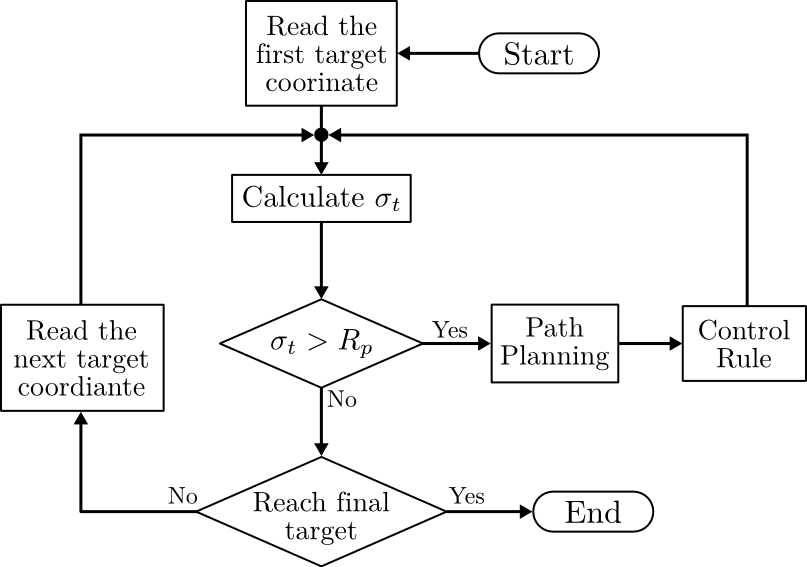
\includegraphics[width=0.8\textwidth]{figures/navigation_flow}
\end{figure}
}

\subsection{Target Angle Calculation}
\subsubsection{Geographic Coordinate System}
\frame{\frametitle{Geographic Coordinate System}
Geographic coordinate system is a reference system used to describe a position on the earth.
There are two kinds of such system: \emph{ECI} and \emph{ECEF}.
\begin{columns}
	\begin{column}{5cm}
		\centering
		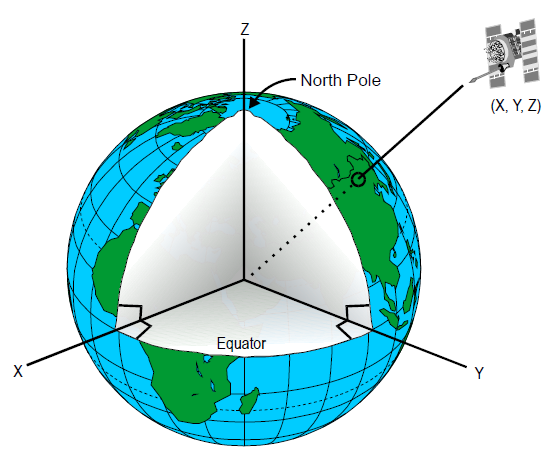
\includegraphics[width=\textwidth]{figures/ECI}

		ECI
	\end{column}
	\begin{column}{5cm}
		\centering
		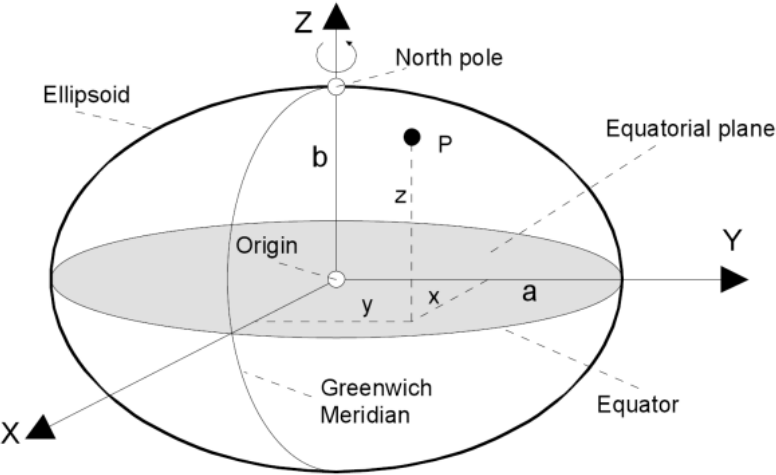
\includegraphics[width=\textwidth]{figures/ECEF}

		ECEF
	\end{column}
\end{columns}
}

\frame{\frametitle{ECEF Ellipsoidal Coordinates}
Ellipsoidal coordinates is the most common coordinate system in describing a position on earth,
which defined by \emph{Latitude} $\phi$, \emph{Longitude} $\lambda$ and \emph{Altitude} $h$.
\begin{figure}
	\centering
	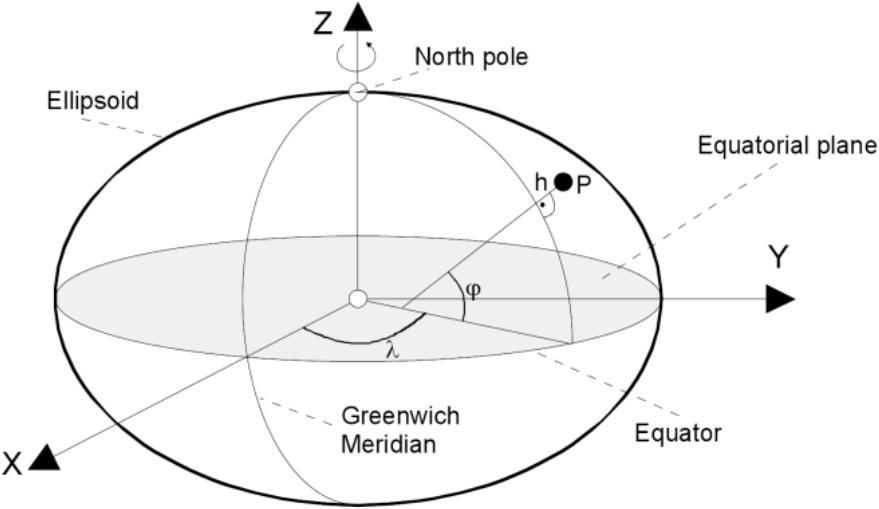
\includegraphics[width=0.7\textwidth]{figures/ellipsoid}
\end{figure}
}

\frame{\frametitle{Datum}
Different definition of ellipsoid will also change its coordinate system,
and the ellipsoid used to define the earth is called a \emph{datum}.
\begin{columns}
	\begin{column}{4cm}
	\centering
		\begin{itemize}
			\item NAD27 \\
			\item NAD83 \\
			\item \emph{WGS84} \\
			\item \ldots \\
		\end{itemize}
	\end{column}
	\begin{column}{6cm}
		\vspace{0.25cm}
		\centering
		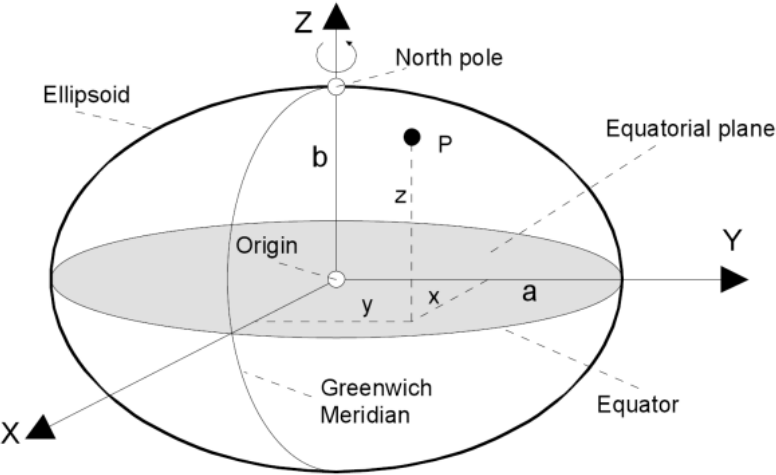
\includegraphics[width=6cm]{figures/ECEF}
	\end{column}
\end{columns}
}

\frame{\frametitle{WGS84 Datum}
WGS84 (World Geodetic System 1984) is the standard ellipsoidal coordinate system used by MTi-G
position sensor and most of the GPS.

\centering
\vspace{1cm}
\begin{tabular}{ | l | c | }
	\hline
	$a$	& $6378137m$ \\ \hline
	$b$	& $6356752.3142m$ \\ \hline
	$f$	& = $(a-b) / a = 1/298.257223563$ \\
	\hline
\end{tabular}
}

\subsubsection{Geodesic}
\frame{\frametitle{Geodesic}
The shortest path between two points on the earth, customarily treated as an ellipsoid of revolution,
is called a \emph{geodesic}. Two geodesic problems are usually considered:
\begin{columns}
	\begin{column}{4cm}
		\begin{enumerate}
			\centering
			\item Direct
			\vspace{0.25cm}
			\item Inverse
		\end{enumerate}
	\end{column}
	\begin{column}{6cm}
		\centering
		\vspace{0.6cm}
		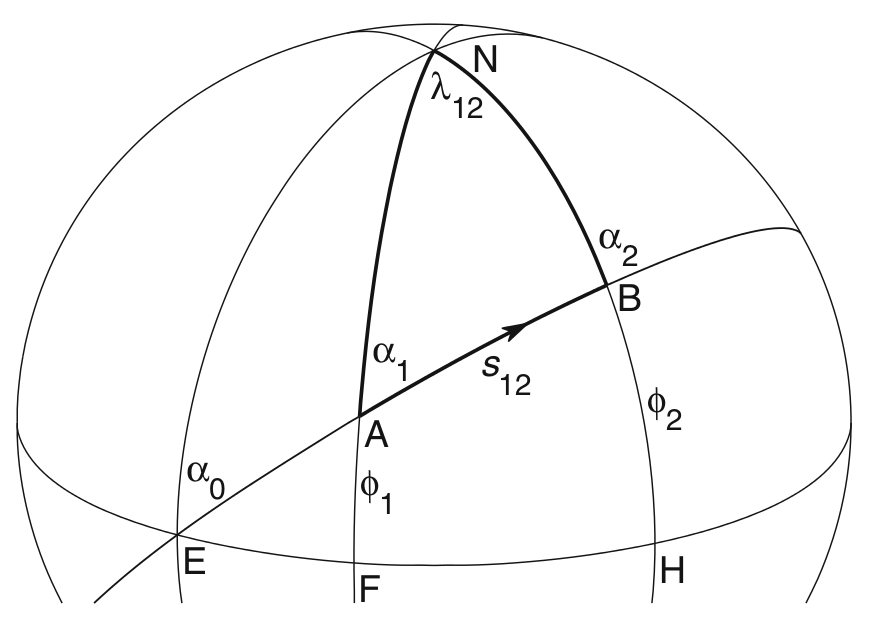
\includegraphics[width=\textwidth]{figures/geodesic}
	\end{column}
\end{columns}
}

\frame{\frametitle{Inverse Problem}
The relative distance and direction between two location is required for autonomous navigation, 
therefore inverse problem in geodesic is considered.
}

\subsubsection{Local Coordinate System}
\frame{\frametitle{Local Tangent Plane}
\emph{Local tangent plane} is the reference system used by AHRS.
\begin{center}
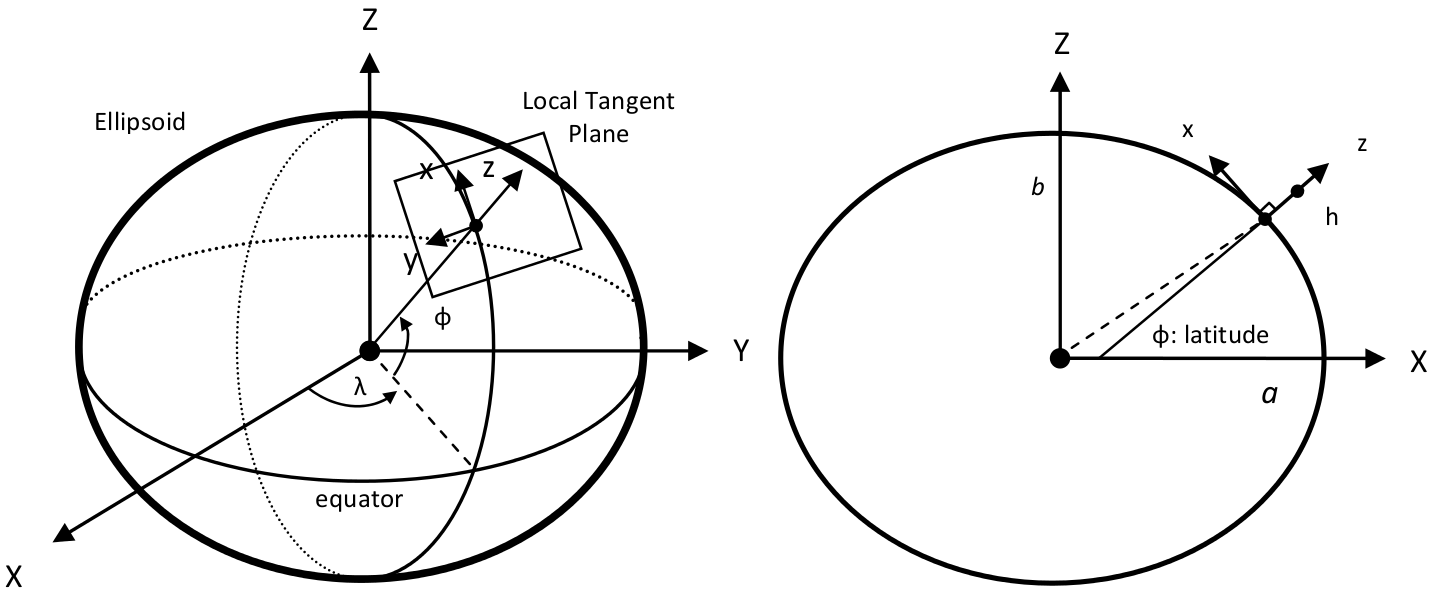
\includegraphics[width=\textwidth]{figures/LTP}
\end{center}
}

\frame{\frametitle{Target Angle}
By the definition of azimuth $\alpha_1$ and yaw $\psi$, 
the target angle $\Theta_t$ relative to robot could be determined:
\begin{columns}
	\begin{column}{5cm}
		\begin{center}
			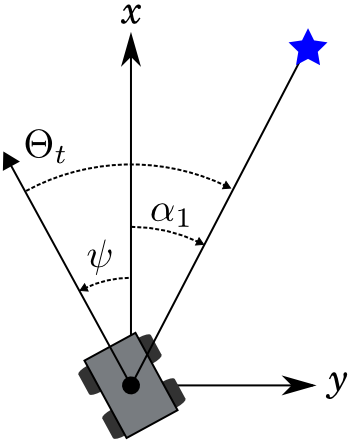
\includegraphics[width=0.7\textwidth]{figures/TargetAngle}
		\end{center}
	\end{column}
	\begin{column}{5cm}
		\begin{equation*}
		\Theta_t = - \alpha_1 - \psi
		\end{equation*}
	\end{column}
\end{columns}
}

\subsection{Path Planning Algorithm}
\subsubsection{Common Obstacle Avoidance Overview}
\frame{\frametitle{Artificial Potential Field}
Artificial Potential Field creates a virtual force field which attracts the robot toward the target,
and retracts it away from the obstacle.
\begin{columns}
	\begin{column}{5cm}
	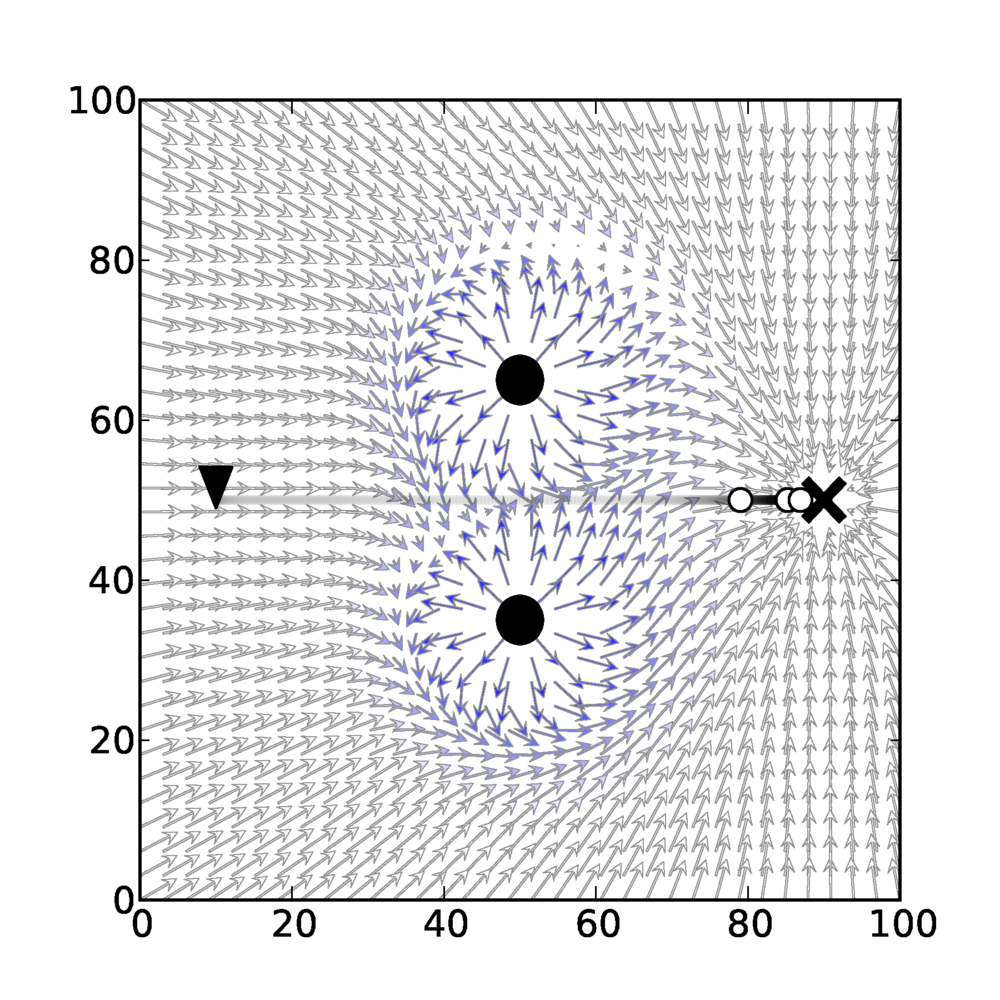
\includegraphics[width=\textwidth]{figures/APF}
	\end{column}
	\begin{column}{5cm}
	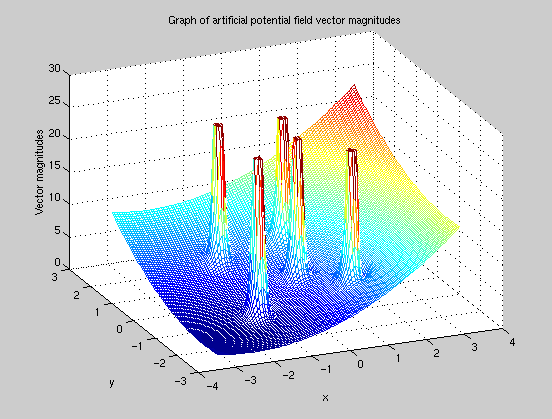
\includegraphics[width=\textwidth]{figures/demo_apf}
	\end{column}
\end{columns}
}

\frame{\frametitle{Artificial Potential Field}
\begin{itemize}
	\item Advantages:
	\begin{itemize}
		\item Global path planning
		\item Efficient Calculation
		\item Easily adapt to the data acquired by LiDAR
	\end{itemize}
	\vspace{0.25cm}
	\item Disadvantages:
	\begin{itemize}
		\item Ignore the kinematic and dynamic constraints
		\item Ignore robot's geometry
	\end{itemize}
\end{itemize}
}

\subsubsection{Vector Field Histogram}
\frame{\frametitle{Vector Field Histogram (VFH)}
VFH generates a polar histogram of the environment around the robot,
identifies wide-enough spaces and calculates corresponding steering direction.
\begin{center}
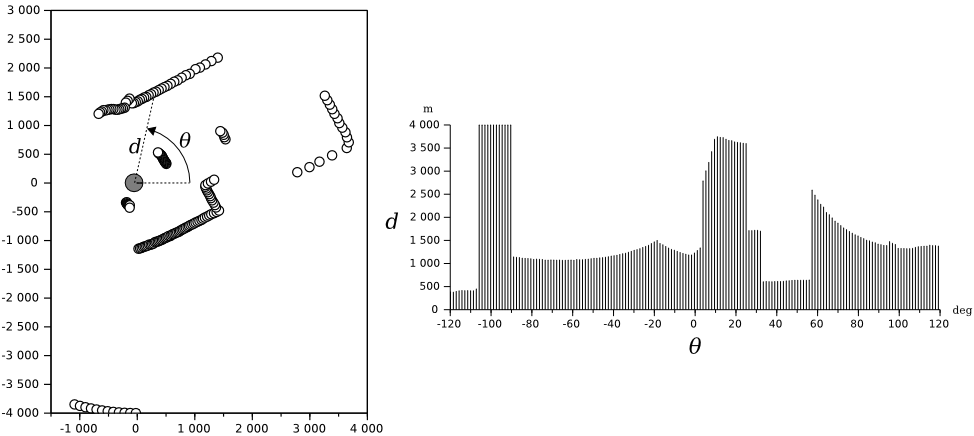
\includegraphics[width=\textwidth]{figures/VFHTotal}
\end{center}
}

\frame{\frametitle{Vector Field Histogram (VFH)}
A cost function $G$ is then applied to every candidate directions,
and the direction which generates the smallest value is then selected:
\begin{equation*}
G = u_{1} \cdot \alpha + u_{2} \cdot \beta + u_{3} \cdot \gamma
\end{equation*}
where
\begin{align*}
	\alpha &= \text{difference between target and candidate direction} \\
	\beta &= \text{difference between current direction and candidate direction} \\
	\gamma &= \text{difference between the previously selected direction and candidate direction}
\end{align*}
$u_{1}$, $u_{2}$ and $u_{3}$ are weighting constants
}

\frame{\frametitle{Vector Field Histogram (VFH)}
\begin{itemize}
	\item Advantages:
	\begin{itemize}
		\item Easily adapt to the data acquired by LiDAR
		\item Efficient Calculation
		\item Adjustable characteristic
	\end{itemize}
	\vspace{0.25cm}
	\item Disadvantages:
	\begin{itemize}
		\item Ignore the kinematic and dynamic constraints
		\item Ignore robot's geometry
		\item \textbf{Direction depends on free-spaces}
	\end{itemize}
\end{itemize}
}

\subsubsection{Curvature Velocity Method}
\frame{\frametitle{Curvature Velocity Method (CVM)}
CVM takes robot's kinematic constraints into account,
assumes it only travels along circular trajectories with curvature $c =  \omega / \nu$,
which uses \emph{velocity space} for path planning.
\begin{figure}
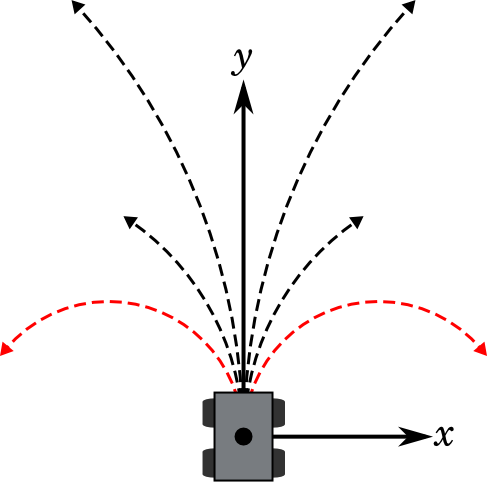
\includegraphics[width=0.4\textwidth]{figures/CVM1}
\end{figure}
}

\frame{\frametitle{Curvature Velocity Method (CVM)}
In order to transform obstacles into velocity space, a distance function $D(c,obs)$
calculates the distance $d$ before collides with obstacle $obs$, along the curvature $c$.
\begin{center}
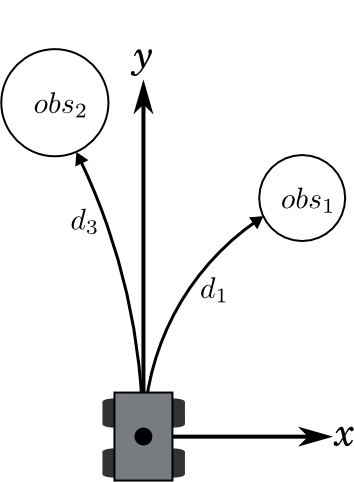
\includegraphics[width=0.35\textwidth]{figures/CVM2}
\end{center}
}

\frame{\frametitle{Curvature Velocity Method (CVM)}
Since the sensor has detection distance, CVM sets a limit $L$ according to its limitation.
Therefore, the distance function $D$ becomes $D_{limit} = min(L,D(c,OBS))$.
\begin{center}
	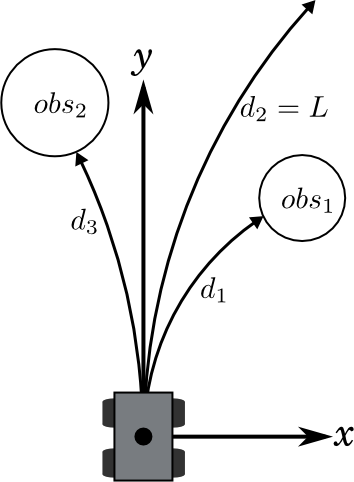
\includegraphics[width=0.35\textwidth]{figures/CVM3}
\end{center}
}

\frame{\frametitle{Curvature Velocity Method (CVM)}
The final decision of new $\omega$ and $\nu$ is made by an object function, which resembles the cost function of previous method:
\begin{equation*}
f(\omega,\nu) = u_{1} \cdot speed(\nu) + u_{2} \cdot dist(\omega,\nu) + u_{3} \cdot head(\omega)
\end{equation*}
where
\begin{align*}
speed(\nu) &= \nu / \nu_{max} \\
dist(\omega,\nu) &= D_{limit}(\frac{\omega}{v},OBS) / L \\
head(\omega) &= 1 - |\theta_{target} - \omega \cdot T_{c} | / \pi \\
\end{align*}
The velocities which generate the largest value will be chosen!
}

\frame{\frametitle{Curvature Velocity Method (CVM)}
\begin{itemize}
	\item Advantages:
	\begin{itemize}
		\item Kinematic and dynamic constraints
		\item Robot's geometry constraint
		\item Adjustable characteristic
	\end{itemize}
	\vspace{0.25cm}
	\item Disadvantages:
	\begin{itemize}
		\item Simplified circular obstacle
		\item \textbf{Velocity sensors are required}
	\end{itemize}
\end{itemize}
}

\subsubsection{Dynamic Window Approaches}
\frame{\frametitle{Dynamic Window Approach (DW)}
DW also assumes the robot only travelled in circular path with rotational velocity $\omega$ and translational velocity $\nu$.
The sensed environment is then transformed into \textbf{velocity space}.
\begin{figure}
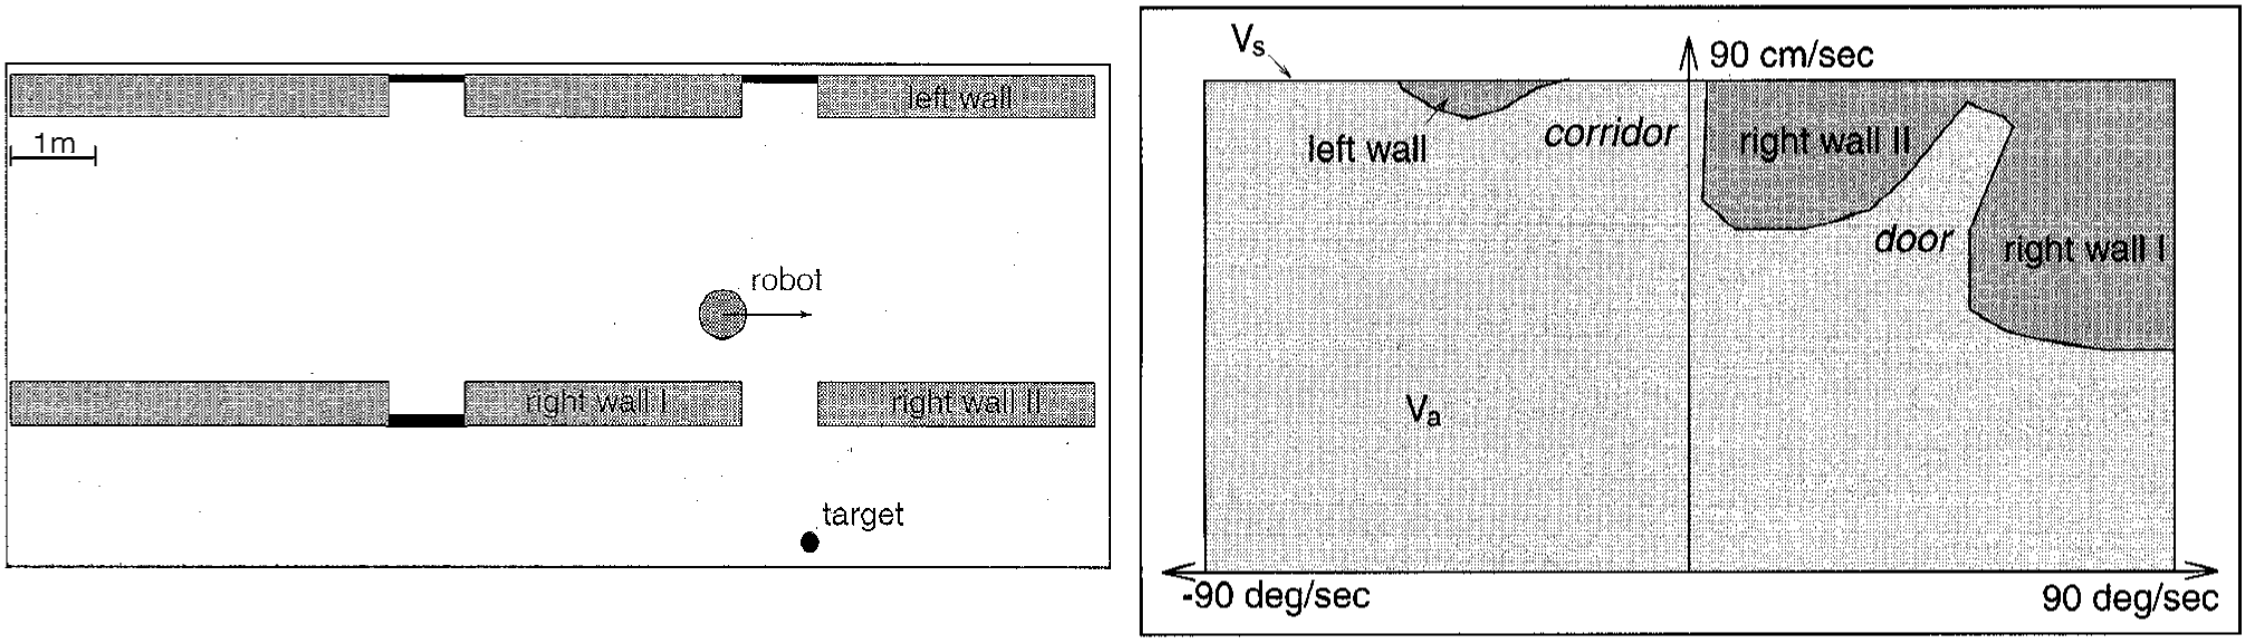
\includegraphics[scale=.17]{figures/DW1}
\end{figure}
}

\frame{\frametitle{Dynamic Window Approach (DW)}
In velocity space, a \emph{dynamic window} is constructed according to its dynamic constraints and current velocities.
Again, an object function is used to choose the optimized velocities.
\begin{figure}
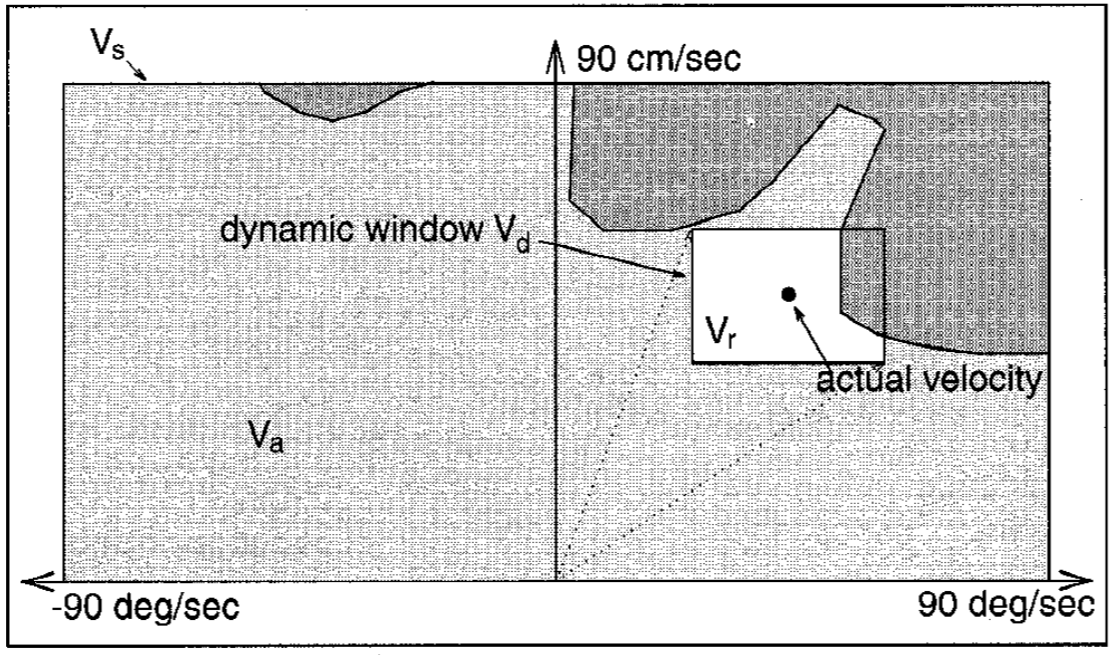
\includegraphics[scale=.25]{figures/DW2}
\end{figure}
}

\frame{\frametitle{Dynamic Window Approach (DW)}
\begin{itemize}
	\item Advantages:
	\begin{itemize}
		\item Kinematic and dynamic constraints
		\item Robot's geometry constraint
		\item Adjustable characteristic
	\end{itemize}
	\vspace{0.25cm}
	\item Disadvantages:
	\begin{itemize}
		\item Complexity
		\item \textbf{Velocity sensors are required}
	\end{itemize}
\end{itemize}
}

\subsection{Vector Field Histogram Plus}
\subsubsection{Introduction}
\frame{\frametitle{Vector Field Histogram Plus (VFH$^{+}$) - Introduction}
VFH$^{+}$ algorithm is an enhanced version of original VFH which offers several improvements:
\begin{enumerate}
	\vspace{0.25cm}
	\item Kinematic constraints
	\vspace{0.25cm}
	\item Robot's geometry constraints
	\vspace{0.25cm}
	\item \textbf{Direction no longer depends on spaces}
\end{enumerate}
}

\frame{\frametitle{VFH$^{+}$ - Four-Stage Process}
The VFH$^{+}$ employs a four-stage data reduction process in order to compute the new direction of motion:
\begin{enumerate}
	\vspace{0.25cm}
	\item Primary Polar Histogram
	\vspace{0.25cm}
	\item Binary Polar Histogram
	\vspace{0.25cm}
	\item Masked Polar Histogram
	\vspace{0.25cm}
	\item Selection of Steering Direcion
	\vspace{0.25cm}
\end{enumerate}
}

\frame{\frametitle{VFH$^{+}$ - with Laser Range Finder}
However, some modification is required in order to implement VFH$^{+}$ with laser range finder, therefore the process become:
\begin{enumerate}
	\vspace{0.25cm}
	\item Primary Polar Histogram
	\vspace{0.25cm}
	\item Identifying Free Spaces
	\vspace{0.25cm}
	\item Blocked Directions
	\vspace{0.25cm}
	\item Selection of Steering Direction
	\vspace{0.25cm}
\end{enumerate}
}

\subsubsection{Algorithm of Steering Direction}
\frame{\frametitle{1: Primary Polar Histogram}
A polar histogram $P_i$ of corresponding measured distance and angle $d_i$ can be generated with following formula:
\begin{equation*}
	P_i = a + b \cdot d_i
\end{equation*}
\begin{center}
	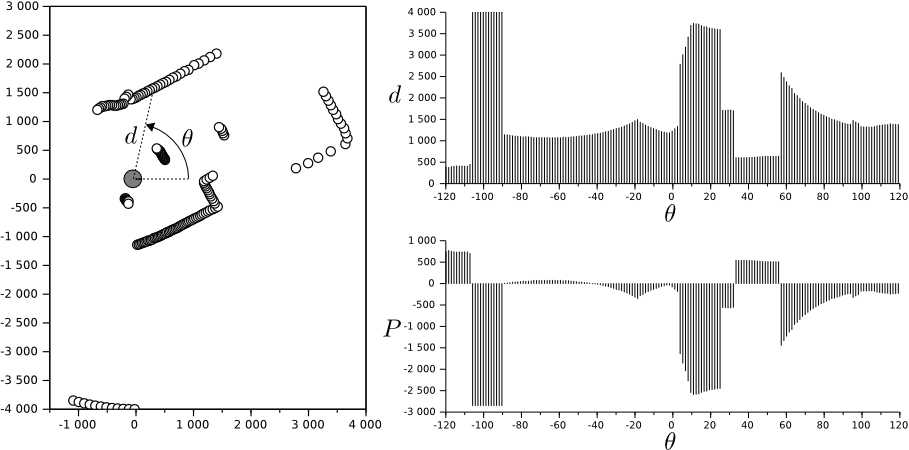
\includegraphics[width=0.9\textwidth]{figures/primary_histogram}
\end{center}
}

\frame{\frametitle{2: Identifying Free Spaces - Boundary Vector}
Both VFH and VFH$^+$ try to identify free spaces $V$ - spaces capable for the robot to pass through,
by different method. Each free space $V_j$ is defined by two boundary vectors $(\mathbf{B_l},\mathbf{B_r})_j$:
\begin{columns}
	\begin{column}{0.4\textwidth}
		\begin{align*}
		\mathbf{B_l}	&= \begin{bmatrix}
					\theta_l & d_l
				   \end{bmatrix} \\
		\mathbf{B_r}	&= \begin{bmatrix}
					\theta_r & d_r
				   \end{bmatrix}
		\end{align*}
	\end{column}
	\begin{column}{0.6\textwidth}
		\begin{center}
			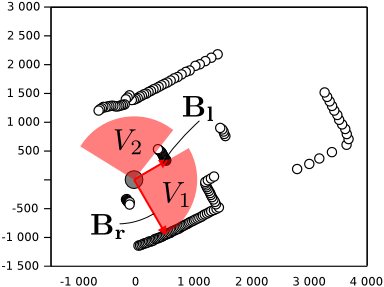
\includegraphics[width=0.9\textwidth]{figures/free_spaces}
		\end{center}
	\end{column}
\end{columns}
}


\frame{\frametitle{2: Identifying Free Spaces - Hysteresis Filter}
VFH$^+$ uses two thresholds $\tau_{max}$ and $\tau_{min}$ instead of single threshold $\tau$ in VFH
to generate a \emph{Binary Histogram} $H_i$, identifying all the free spaces.
\[
H_i = 
\begin{cases}
	1	& \textrm{if } P_i \geq \tau_{max} \\
	0	& \textrm{if } P_i \leq \tau_{min} \\
	H_{i-1}	& \textrm{otherwise}
\end{cases}
\]
}

\frame{\frametitle{2: Identifying Free Spaces - Hysteresis Filter}
By hysteresis filter, VFH$^+$ has reduced the number of free spaces, which overcomes the frequent oscillations
of VFH in narrow indoor environment.
\begin{center}
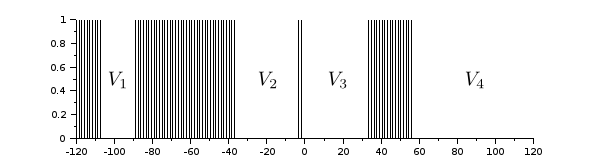
\includegraphics[width=0.85\textwidth]{figures/binary_histogram_1}

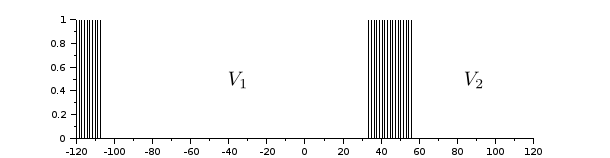
\includegraphics[width=0.85\textwidth]{figures/binary_histogram_2}
\end{center}
}

\frame{\frametitle{2: Free Spaces - Robot's Geometry}
With geometry constraints, free spaces with shrinked boundaries
$\hat{V_j} = (\hat{\mathbf{B_l}},\hat{\mathbf{B_r}})_j$ of each $V_j$ is calculated:
\begin{columns}
	\begin{column}{0.5\textwidth}
		\begin{align*}
			\hat{\mathbf{B_l}}	&= \begin{bmatrix}
							\theta_l - \delta_l & d_l\cos\delta_l
						   \end{bmatrix} \\
			\hat{\mathbf{B_r}}	&= \begin{bmatrix}
							\theta_r + \delta_r & d_r\cos\delta_r
						   \end{bmatrix}
			\intertext{where}
			\delta_l &= \arcsin(\frac{w_s}{d_l}) \\
			\delta_r &= \arcsin(\frac{w_s}{d_r})
		\end{align*}
	\end{column}
	\begin{column}{0.5\textwidth}
		\begin{figure}
			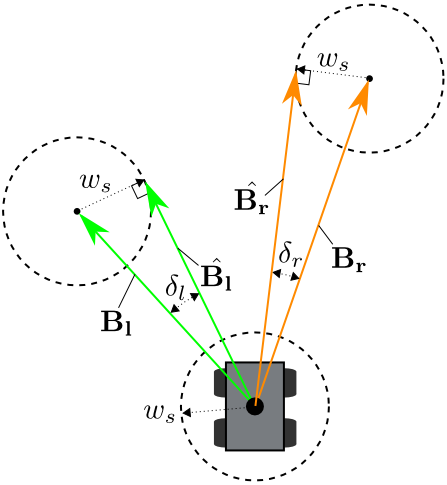
\includegraphics[width=\textwidth]{figures/width}
		\end{figure}
	\end{column}
\end{columns}
}

\frame{\frametitle{2: Free Spaces - Boundary Overlapped}
The $V_j'$ with overlapped boundaries where $\theta_r + \delta_r > \theta_l - \delta_l$ are abandoned, since they are considered too narrow to pass through.
\begin{center}
	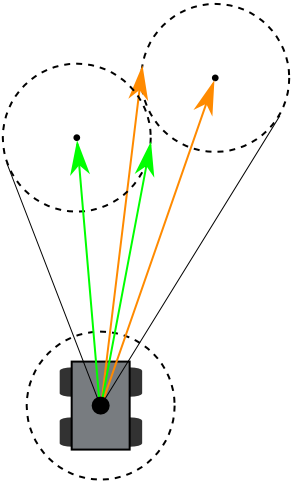
\includegraphics[width=0.3\textwidth]{figures/width_overlapped}
\end{center}
}

\frame{\frametitle{3: Blocked Directions}
VFH$^+$ takes the minimum radius of rotation of robot into account,
determines the limitation of steering angles $\phi_r$ and $\phi_l$.
\begin{center}
	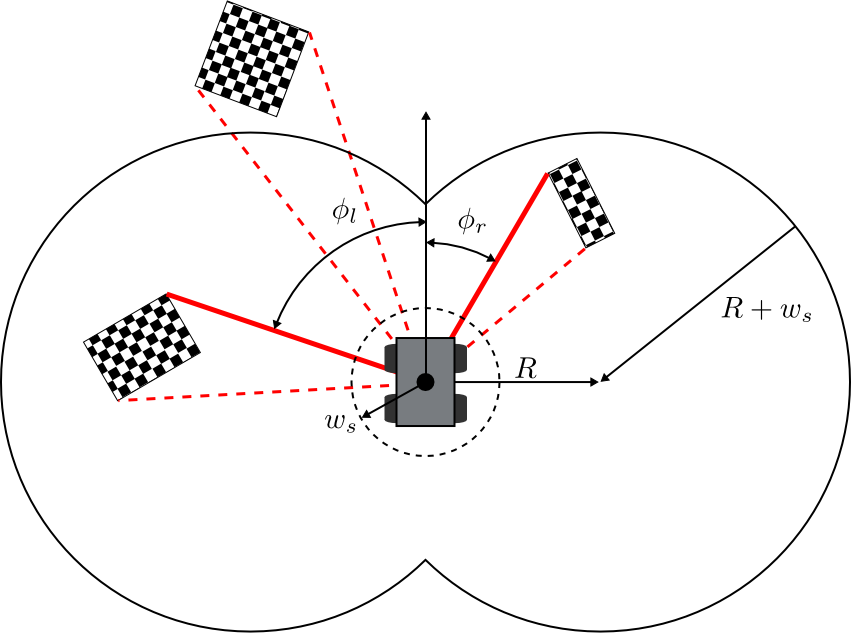
\includegraphics[width=0.65\textwidth]{figures/blocked_directions}
\end{center}
}

\frame{\frametitle{3. Blocked Directions - Detection Histogram}
In order to calculate $\phi_r$ and $\phi_l$, the detection histogram $D_i$ is generated first:
\begin{equation*}
	D_i = |R\sin\theta_i| + \sqrt{R^2\sin^2\theta_i + w_s^2 + 2Rw_s}
\end{equation*}
\begin{center}
	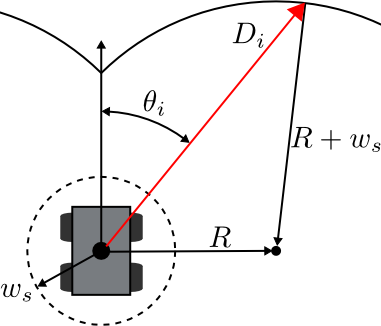
\includegraphics[width=0.45\textwidth]{figures/detection_histogram}
\end{center}
}

\frame{\frametitle{3. Blocked Directions - Masked Histogram}
The masked histogram $M_i = d_i - D_i$ shows whethter the steering angle is blocked by obstacles.
\begin{figure}
	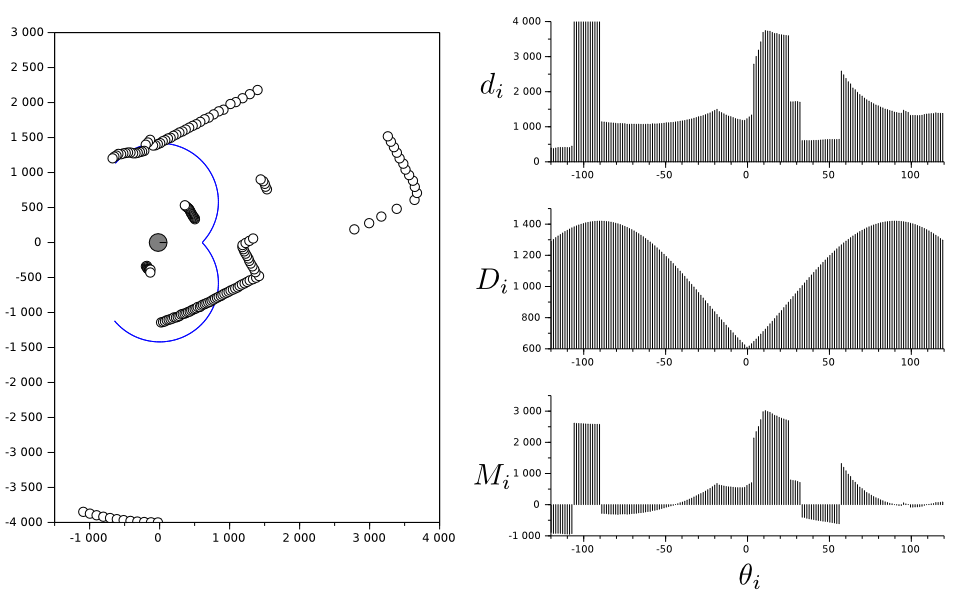
\includegraphics[width=0.9\textwidth]{figures/histogram_transform}
\end{figure}
}

\frame{\frametitle{3. Blocked Directions - Determine $\phi_r$ and $\phi_l$}
$\phi_r$ and $\phi_l$ can be efficiently found by following method: \\
\vspace{0.25cm}
\textrm{1) Initially set }$\phi_r = -\pi$\textrm{ and }$\phi_l = \pi$ \\
\vspace{0.25cm}
\textrm{2) For every }$M_i < 0$\textrm{:} \\
\vspace{0.25cm}
\hspace{0.4cm} \textrm{a) If }$\theta_i < 0$\textrm{ and }$\theta_i > \phi_r$\textrm{ , set }$\phi_r$\textrm{ to }$\theta_i$ \\
\vspace{0.25cm}
\hspace{0.4cm} \textrm{a) If }$\theta_i > 0$\textrm{ and }$\theta_i < \phi_l$\textrm{ , set }$\phi_l$\textrm{ to }$\theta_i$ \\
}

\frame{\frametitle{4. Selection of Steering Direction - Width of Free Spaces}
According to the width of each free space $\hat{V_j}$, single or multiple candidate directions $c$ could be found.
The width of a free space is determined by its spanning angle $\epsilon = \theta_l - \theta_r$ and a threshold $\tau_a$,
which has 3 kinds of different situation:
\begin{center}
	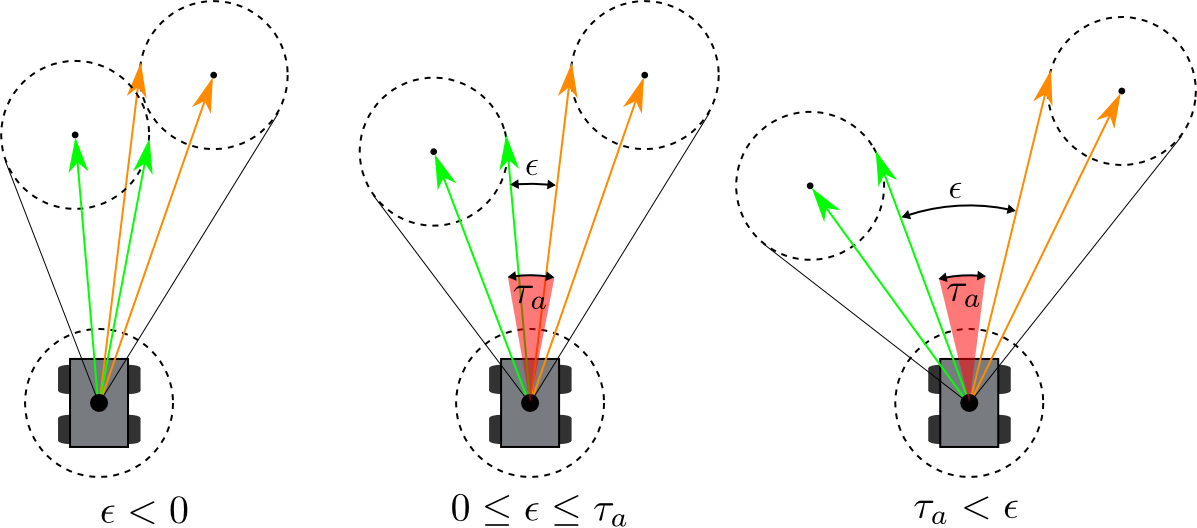
\includegraphics[width=\textwidth]{figures/epsilon_situation}
\end{center}
}

\frame{\frametitle{4. Selection of Steering Direction - Candidate Directions}
$\epsilon < 0$ represents free space with overlapped boundary, which is abandoned.
\begin{columns}
	\begin{column}{0.4\textwidth}
		\begin{itemize}
			\item No candidate direction! \\
		\end{itemize}
	\end{column}
	\begin{column}{0.6\textwidth}
		\begin{center}
			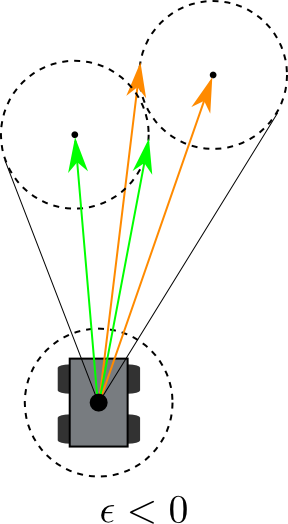
\includegraphics[width=0.4\textwidth]{figures/epsilon_situation_1}
		\end{center}
	\end{column}
\end{columns}
}

\frame{\frametitle{4. Selection of Steering Direction - Candidate Directions}
For a free space with $0 \leq \epsilon \leq \tau_a$,
the centered direction is the only candidate direction.
\begin{columns}
	\begin{column}{0.4\textwidth}
		\begin{itemize}
			\item $c_n = \frac{\theta_l + \theta_r}{2}$ \\
		\end{itemize}
	\end{column}
	\begin{column}{0.6\textwidth}
		\begin{center}
			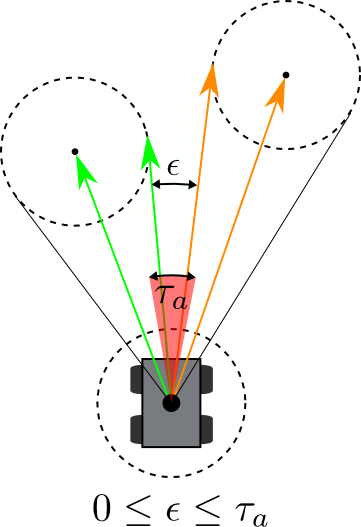
\includegraphics[width=0.5\textwidth]{figures/epsilon_situation_2}
		\end{center}
	\end{column}
\end{columns}
}

\frame{\frametitle{4. Selection of Steering Direction - Candidate Directions}
For a free space with $0 < \tau_a < \epsilon$, there are 2 or 3 candidate directions.
\begin{columns}
	\begin{column}{0.4\textwidth}
		\begin{itemize}
			\item $c_r = \theta_r$ \\
			\item $c_l = \theta_l$ \\
			\item If $\theta_l < \Theta_t < \theta_r$, \\
				$c_t = \Theta_t$ \\
		\end{itemize}
	\end{column}
	\begin{column}{0.6\textwidth}
		\begin{center}
			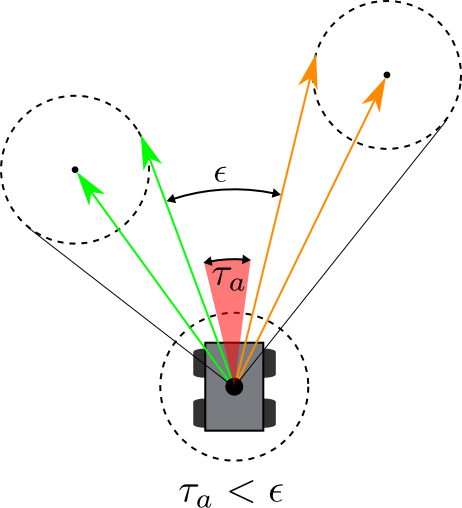
\includegraphics[width=0.7\textwidth]{figures/epsilon_situation_3}
		\end{center}
	\end{column}
\end{columns}
}

\frame{\frametitle{4. Selection of Steering Direction - Cost Function}
Like VFH, VFH$^+$ also uses a cost function to select the preferred direction $c_t$:
\begin{align*}
	G(c) &= \mu_1 \cdot (|c - \Theta_t|) + \mu_2 \cdot |c| + \mu_3 \cdot (|c - c_{t-1}|) \\
	\intertext{and}
	c_t &= min \left\{ G(c) \right\} \\
	\intertext{where}
	\Theta_t &= \text{Target direction} \\
	c &= \text{Candidate directions} \\
	c_{t-1} &= \text{Previously selected direction} \\
\end{align*}
}

\frame{\frametitle{No Candidate Directions!}
\begin{columns}
	\begin{column}{0.5\textwidth}
		\begin{center}
			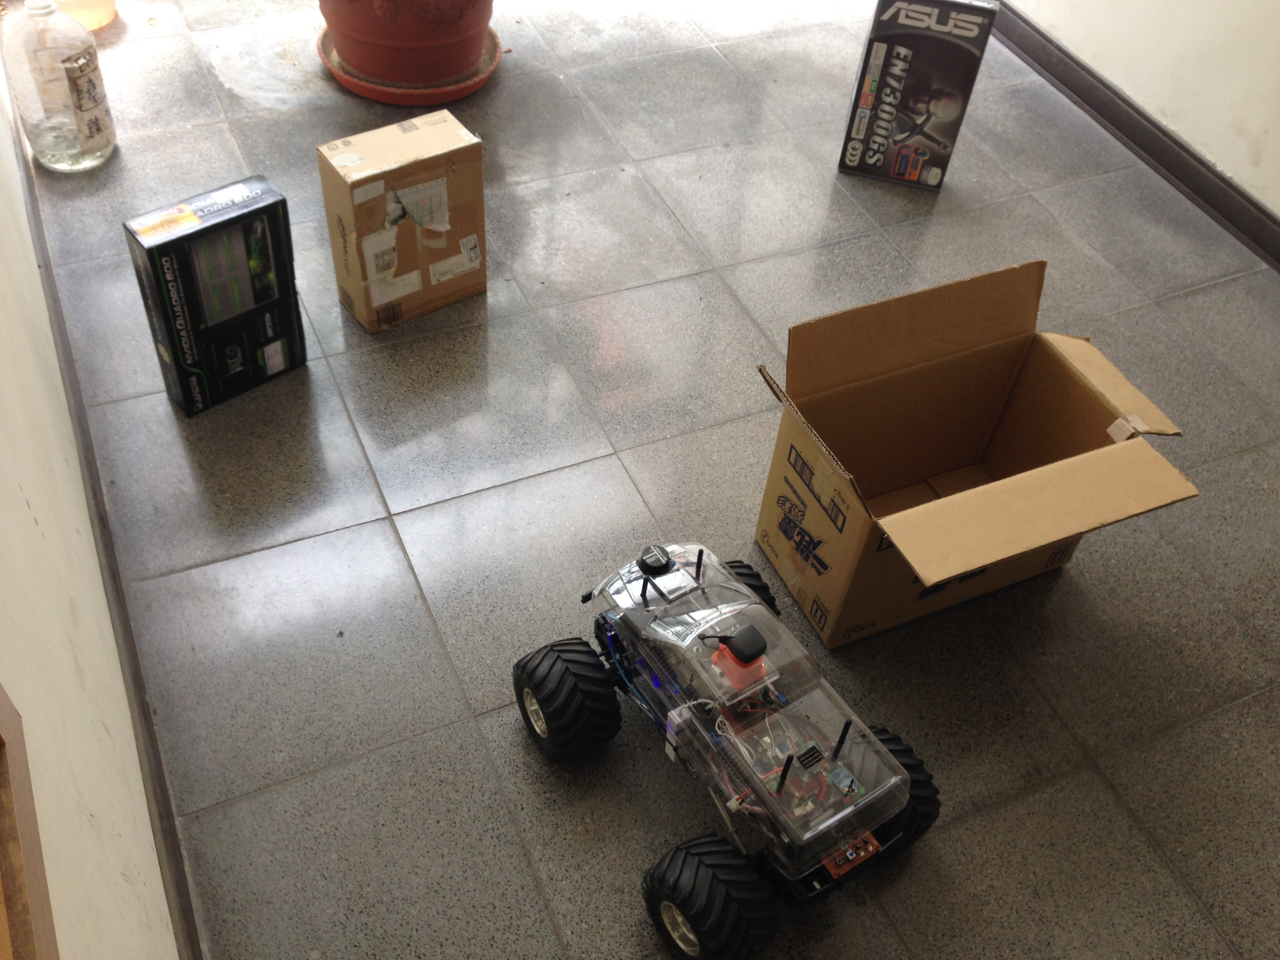
\includegraphics[width=\textwidth]{figures/NoWayToGo_Real}
		\end{center}
	\end{column}
	\begin{column}{0.5\textwidth}
		\begin{center}
			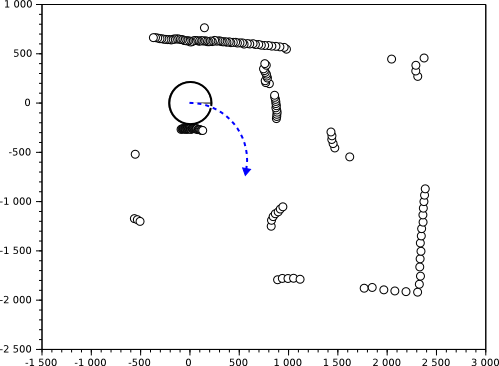
\includegraphics[width=\textwidth]{figures/NoWayToGo}
		\end{center}
	\end{column}
\end{columns}
}

\subsection{Algorithm of Speed}
\subsubsection{Obstacle Density}

\frame{\frametitle{Obstacle Density Function}
VFH$^+$ uses \emph{Obstacle density function} $D$ to calculate the speed of robot in the environment:

\[
	D(d_i) = 1 - \frac{1}{N}\sum_{i=1}^{N}{\frac{d_i}{d_{max}}}
\]

The value of $D$ lies between $0$ and $1$. Therefore, defined a maximum speed $v_{max}$
and minimum speed $v_{min}$, the speed of robot in the environment $v$ could be determined:

\[
	v = v_{min} + (1 - D(d_i)) \cdot (v_{max} - v_{min})
\]
}

\frame{\frametitle{Obstacle Density Function}
\begin{columns}
	\begin{column}{0.5\textwidth}
		\begin{center}
			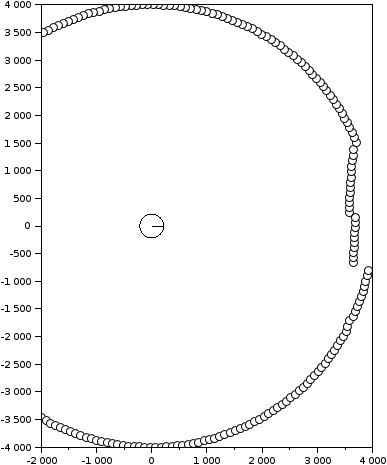
\includegraphics[width=0.9\textwidth]{figures/density_1}

			$D = 0.01$
		\end{center}
	\end{column}
	\begin{column}{0.5\textwidth}
		\begin{center}
			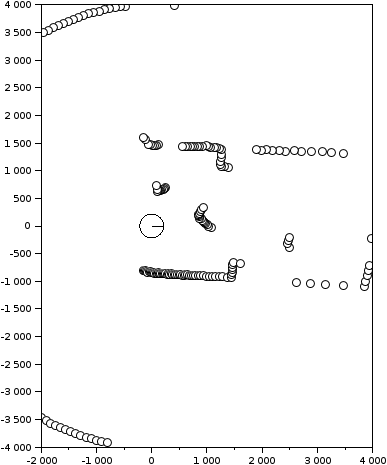
\includegraphics[width=0.9\textwidth]{figures/density_2}

			$D = 0.49$
		\end{center}
	\end{column}
\end{columns}
}

\frame{\frametitle{Obstacle Approaching Rate}
Speed controlled by $D$ considered only current environment, which is insufficient for high speed robot.
Therefore, \emph{Obstacle approaching rate} $\delta$ is introduced:

\[
\delta = -\frac{1}{N}\sum_j{\frac{(d_j)_t - (d_j)_{t-1}}{T}}
\]

\begin{center}
	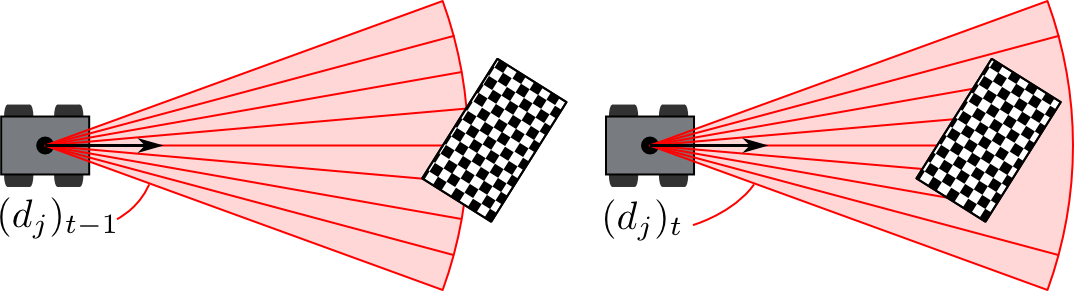
\includegraphics[width=\textwidth]{figures/obstacle_approaching_rate}
\end{center}
}

\frame{\frametitle{Obstacle Approaching Rate}
For high speed robot, the ability of deceleration while approaching an obstacle with high speed is critical.
Therefore only \emph{approaching} rate of change is considered:
\[
	\delta_a = -\frac{1}{N}\sum_j{\frac{P((d_j)_t - (d_j)_{t-1})}{T}}
\]

where
\[
	P(x) = 
	\begin{cases}
		x	& \textrm{if } x < 0 \\
		0	& \textrm{otherwise} \\
	\end{cases}
\]
}

\frame{\frametitle{Obstacle Approaching Rate}
In order to combine obstacle approaching rate with obstacle density,
it has to be normalize to the range between $0$ and $1$ with maximum speed $v_{max}$:
\[
	\delta_n = -\frac{1}{N \cdot v_{max}}\sum_j{\frac{P((d_j)_t - (d_j)_{t-1})}{T}}
\]

And the speed $v$ becomes:
\[
	v = v_{min} + (1-\frac{D(d_i)+\delta_n}{2}) \cdot (v_{max} - v_{min})
\]
}	
\subsubsection{Conclusion}
\frame{\frametitle{Conclusion}
Compare to original VFH method, VFH$^+$ eventually overcomes some defects:
\begin{itemize}
	\item Overcome the primary problem of VFH where steering angle is determined by spaces
	\item Create smooth trajectory by hysteresis threshold
	\item Take robot's geometry and kinematic constraints into account
\end{itemize}
\vspace{0.25cm}
However, it still suffers from some problems:
\begin{itemize}
	\item The geometry of the robot is assumed to be circular
	\item Leads the robot into dead end which can be avoided
\end{itemize}
}

\end{document}
